% $Header: /cvsroot/latex-beamer/latex-beamer/solutions/conference-talks/conference-ornate-20min.en.tex,v 1.6 2004/10/07 20:53:08 tantau Exp $

\documentclass{beamer}

\mode<presentation>
{
%  \usetheme{Hannover}
\usetheme[width=0.7in]{Hannover}
% or ...

  \setbeamercovered{transparent}
  % or whatever (possibly just delete it)
}
\usepackage{longtable}
\usepackage{booktabs}
%\usepackage{qtree}

\usepackage[english]{babel}
% or whatever

\usepackage[latin1]{inputenc}
% or whatever

\usepackage{times}
%\usepackage[T1]{fontenc}
% Or whatever. Note that the encoding and the font should match. If T1
% does not look nice, try deleting the line with the fontenc.
%\usepackage{logictheme}

\usepackage{multirow}
\usepackage{totpages}
\usepackage{hyperref}
\usepackage{booktabs}
\usepackage[round]{natbib}

\usepackage{listings}
\lstset{frame=none, showstringspaces=false, basicstyle=\ttfamily\bfseries\footnotesize,
  xleftmargin=-8mm,language=Haskell,breaklines=true}

\usepackage{tikz}
\usetikzlibrary{positioning}
\usepackage{viking}

\usepackage{pifont}
\usepackage{amsmath,amsfonts,xspace,xcolor,url}
\newcommand{\cross}{\ding{55}}

\newcommand{\blt}{- } %used for bullets in a list

\newcounter{datadefnum} %Datadefinition Number
\newcommand{\ddthedatadefnum}{DD\thedatadefnum}
\newcommand{\ddref}[1]{DD\ref{#1}}

\newcommand{\colAwidth}{0.1\textwidth}
\newcommand{\colBwidth}{0.8\textwidth}

\renewcommand{\arraystretch}{1.1} %so that tables with equations do not look crowded

\pgfdeclareimage[height=0.7cm]{logo}{McMasterLogo}
\title[\pgfuseimage{logo}] % (optional, use only with long paper titles)
{A Literate Approach for Improving the Verifiability, Reusability and
  Reproducibility of Scientific Computing Software}

%\subtitle
%{Include Only If Paper Has a Subtitle}

\author[Slide \thepage~of \pageref{TotPages}] % (optional, use only with lots of
                                              % authors)
{\textbf{Spencer Smith}, Jacques Carette, Dan Szymczak, Steven Palmer}
% - Give the names in the same order as the appear in the paper.
% - Use the \inst{?} command only if the authors have different
%   affiliation.

\institute[McMaster University] % (optional, but mostly needed)
{
  Computing and Software Department\\
  Faculty of Engineering\\
  McMaster University
}
% - Use the \inst command only if there are several affiliations.
% - Keep it simple, no one is interested in your street address.

\date[Jan 12, 2016] % (optional, should be abbreviation of conference name)
{CAIMS 2017, Third Canadian Symposium in Numerical Analysis and Scientific
Computing (CSNASC): Simulation, July 18, 2017}
% - Either use conference name or its abbreviation.
% - Not really informative to the audience, more for people (including
%   yourself) who are reading the slides online

\subject{computational science and engineering, software engineering, software
  quality, literate programming, software requirements specification, document
  driven design}
% This is only inserted into the PDF information catalog. Can be left
% out. 

% If you have a file called "university-logo-filename.xxx", where xxx
% is a graphic format that can be processed by latex or pdflatex,
% resp., then you can add a logo as follows:

%\pgfdeclareimage[height=0.5cm]{Mac-logo}{McMasterLogo}
%\logo{\pgfuseimage{Mac-logo}}

% Delete this, if you do not want the table of contents to pop up at
% the beginning of each subsection:
% \AtBeginSubsection[]
% {
%   \begin{frame}<beamer>
%     \frametitle{Outline}
%     \tableofcontents[currentsection,currentsubsection]
%   \end{frame}
% }

% If you wish to uncover everything in a step-wise fashion, uncomment
% the following command: 

%\beamerdefaultoverlayspecification{<+->}

\beamertemplatenavigationsymbolsempty 

% have SRS and LP open during the presentation

\begin{document}

%%%%%%%%%%%%%%%%%%%%%%%%%%%%%%%%%%%%%%
\hoffset=-.4in %removing side bar for these frames
\begin{frame}[plain]

\titlepage

\end{frame}
\hoffset=0in %restore
%%%%%%%%%%%%%%%%%%%%%%%%%%%%%%%%%%%%%%

% \begin{frame}

% \frametitle{Literate Scientific Software}
% \tableofcontents
% % You might wish to add the option [pausesections]

% % make like a story - the phases - reason for, why works, advantages
% % changing the history a bit to make a more rational narrative

% \end{frame}

%%%%%%%%%%%%%%%%%%%%%%%%%%%%%%%%%%%%%%

\begin{frame}

\frametitle{Abstract}

\begin{itemize}
\item \textbf{Goal} -- Improve quality of SCS
\item \textbf{Idea} -- Adapt ideas from SE
\item \textbf{Document Driven Design}
\begin{itemize}
\item Good -- improves quality
\item Bad -- ``manual'' approach is too much work
\end{itemize}
\item \textbf{Solution}
\begin{itemize}
\item Capture knowledge
\item Generate all things
\item Avoid duplication
\item Traceability
\end{itemize}
\item \textbf{Showing great promise}
\begin{itemize}
\item Significant work yet to do
\item Looking for examples/partners
\end{itemize}
\end{itemize}

\end{frame}

%%%%%%%%%%%%%%%%%%%%%%%%%%%%%%%%%%%%%%

\section[Scope]{Scope}

%%%%%%%%%%%%%%%%%%%%%%%%%%%%%%%%%%%%%%

%\hoffset=-.4in
\begin{frame}[plain, fragile]

\frametitle{Scope: Large/Multiyear} %replace with pictures

\begin{tikzpicture}[remember picture,overlay]
\node [xshift=0cm,yshift=0.15cm] at (current page.center)
{
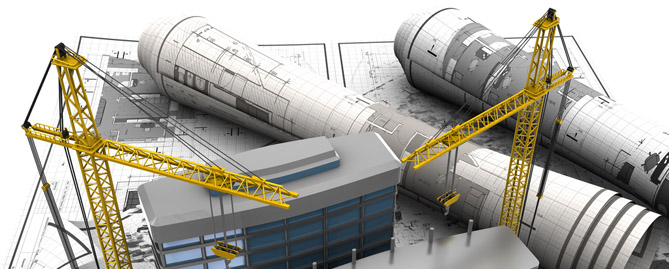
\includegraphics[width=1.15\textwidth]{MSc_CE.jpg}
};
\end{tikzpicture}

\end{frame}
\hoffset=0in

%%%%%%%%%%%%%%%%%%%%%%%%%%%%%%%%%%%%%%

%\hoffset=-.8in
\begin{frame}[plain, fragile]

\frametitle{Scope: Program Families}

% if time add another program family example

\begin{tikzpicture}[remember picture,overlay]
\node [xshift=0cm,yshift=-3.cm] at (current page.center)
{
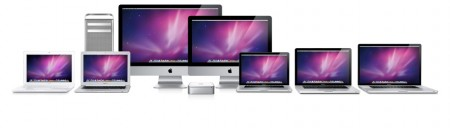
\includegraphics[width=1.2\textwidth]{apple-mac-products-450x128.jpg}
};
\end{tikzpicture}

\begin{tikzpicture}[remember picture,overlay]
\node [xshift=0cm,yshift=1.cm] at (current page.center)
{
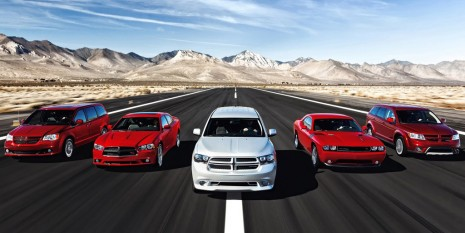
\includegraphics[width=0.8\textwidth]{dodge-lineup.jpg}
};
\end{tikzpicture}

\end{frame}
\hoffset=0in

%%%%%%%%%%%%%%%%%%%%%%%%%%%%%%%%%%%%%%

%\hoffset=-.8in
\begin{frame}[plain, fragile]

\frametitle{Scope: End User Developers} 
% end user developers solving physics problems

\begin{tikzpicture}[remember picture,overlay]
\node [xshift=0cm,yshift=-0.2cm] at (current page.center)
{
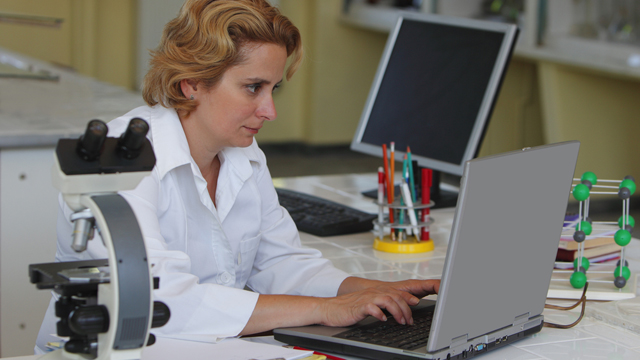
\includegraphics[width=1\textwidth]{ScientistAtAComputer.jpg}
};
\end{tikzpicture}

\end{frame}
\hoffset=0in

%%%%%%%%%%%%%%%%%%%%%%%%%%%%%%%%%%%%%%

%\hoffset=-.8in
\begin{frame}[plain, fragile]

\frametitle{Scope: Physical Science} %replace with pictures

\begin{tikzpicture}[remember picture,overlay]
\node [xshift=3.75cm,yshift=0.9cm] at (current page.center)
{
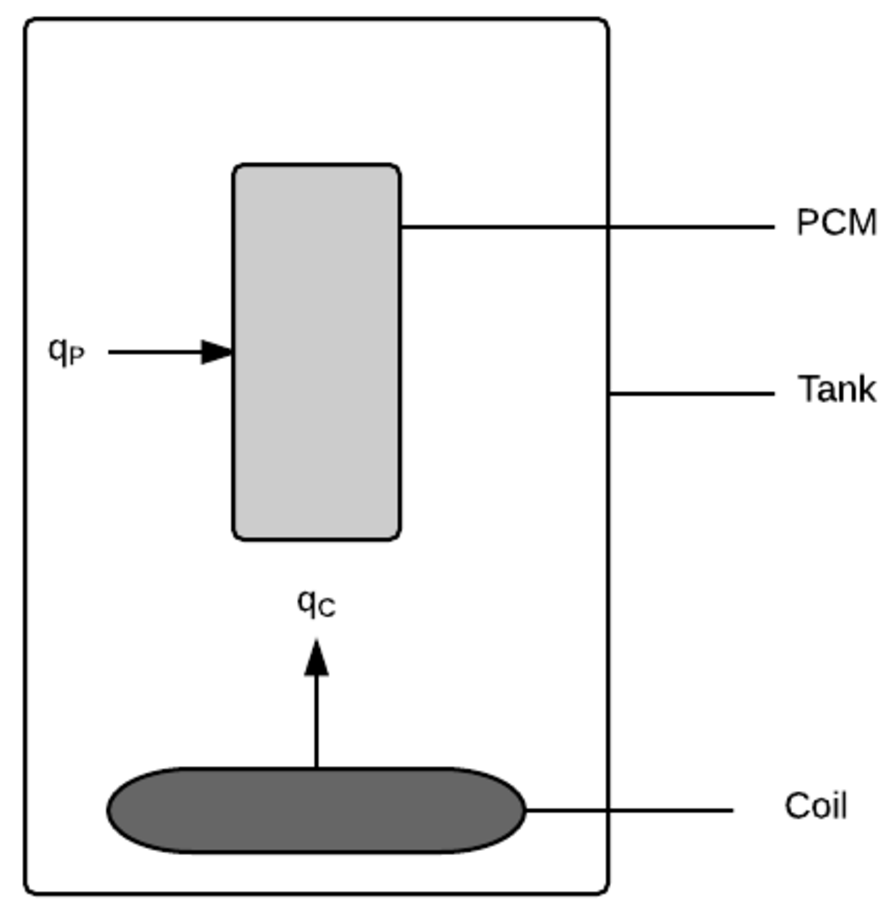
\includegraphics[width=0.4\textwidth]{Tank.pdf}
};
\end{tikzpicture}

\begin{tikzpicture}[remember picture,overlay]
\node [xshift=-3.5cm,yshift=1.55cm] at (current page.center)
{
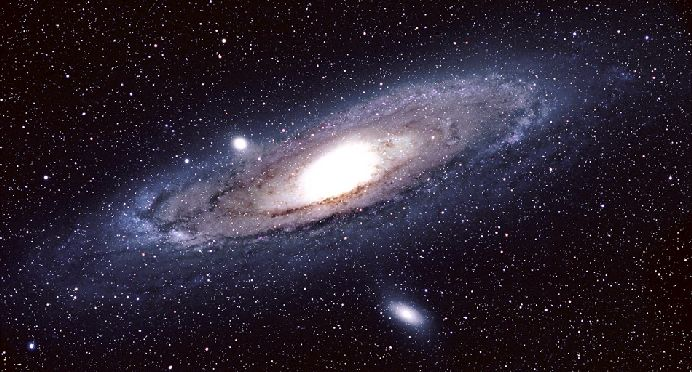
\includegraphics[width=0.5\textwidth]{m31_jg.jpg}
};
\end{tikzpicture}

\begin{tikzpicture}[remember picture,overlay]
\node [xshift=0.1cm,yshift=0.8cm] at (current page.center)
{
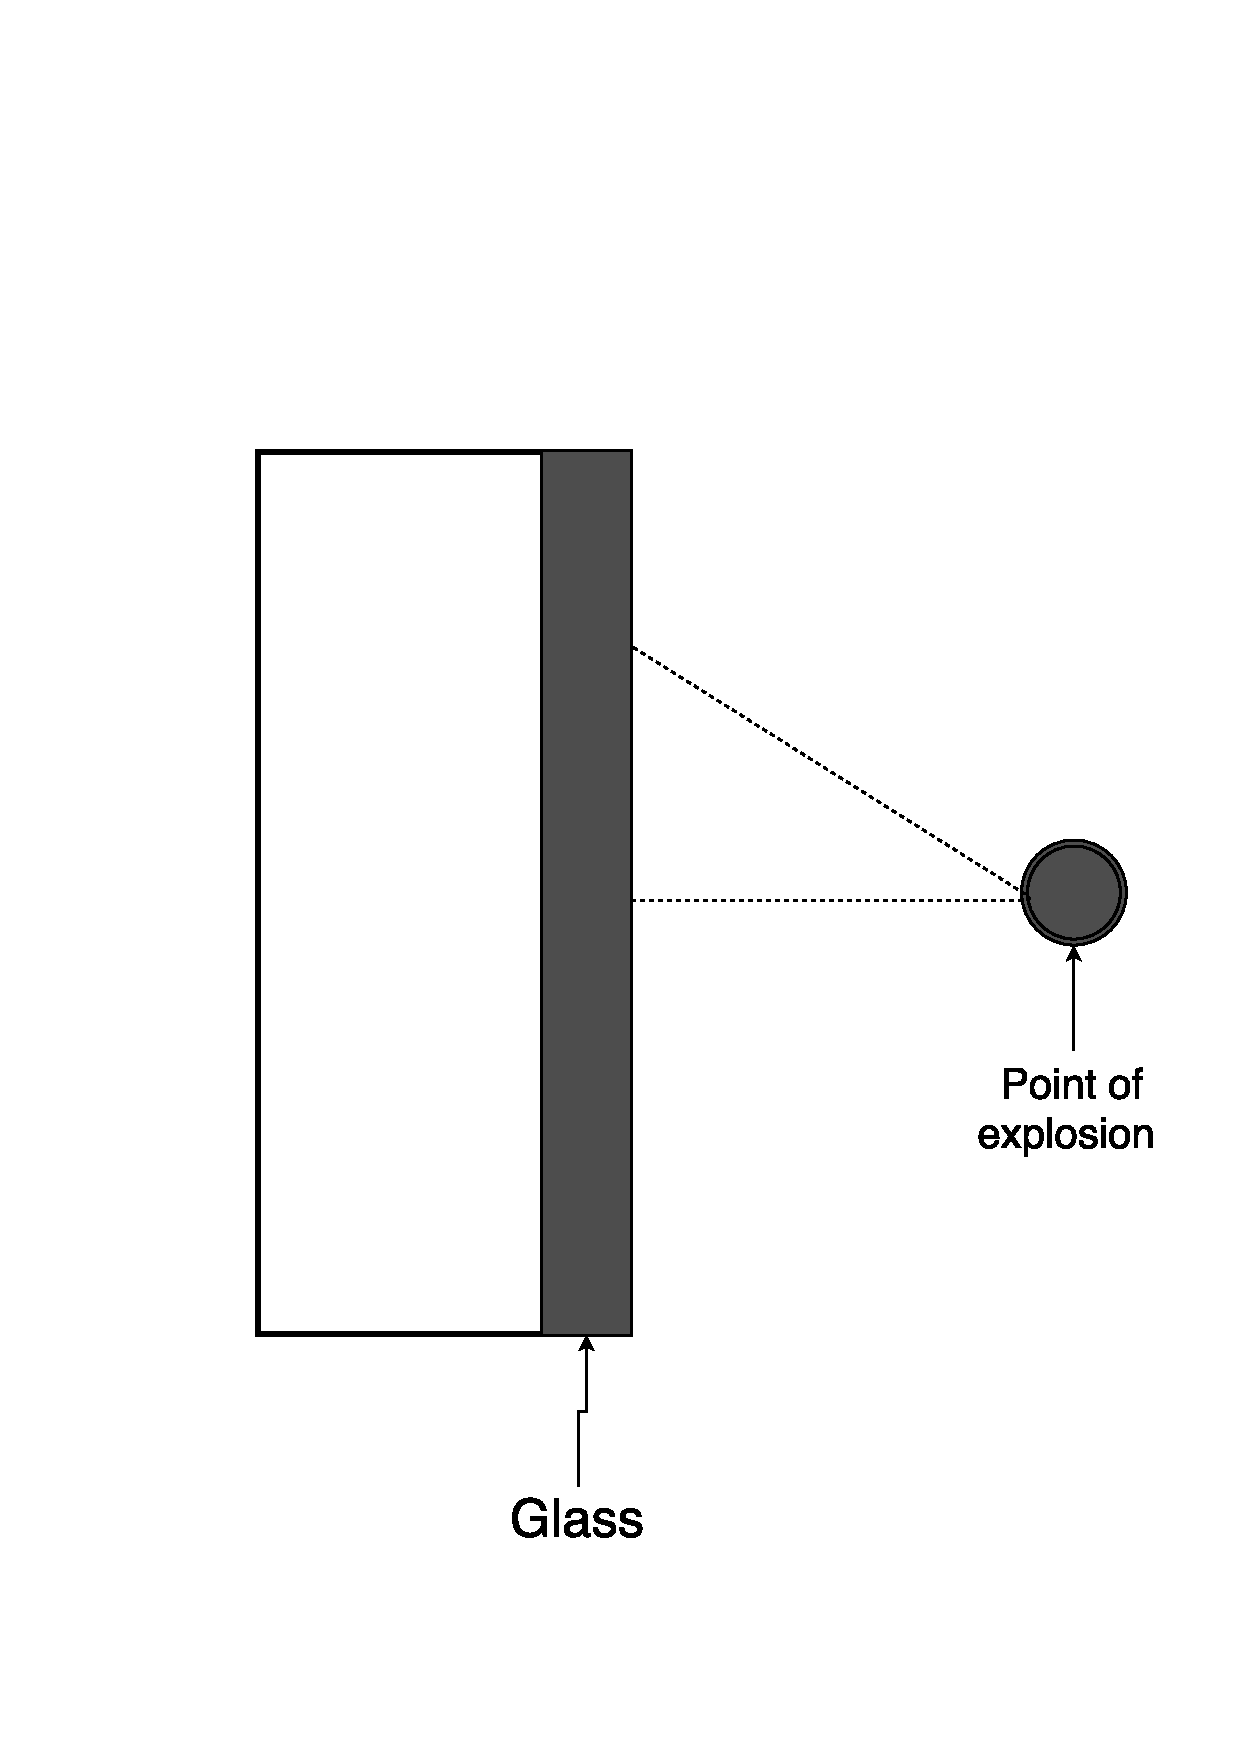
\includegraphics[width=0.3\textwidth]{physicalsystimage.pdf}
};
\end{tikzpicture}

\begin{tikzpicture}[remember picture,overlay]
\node [xshift=-3.5cm,yshift=-2.25cm] at (current page.center)
{
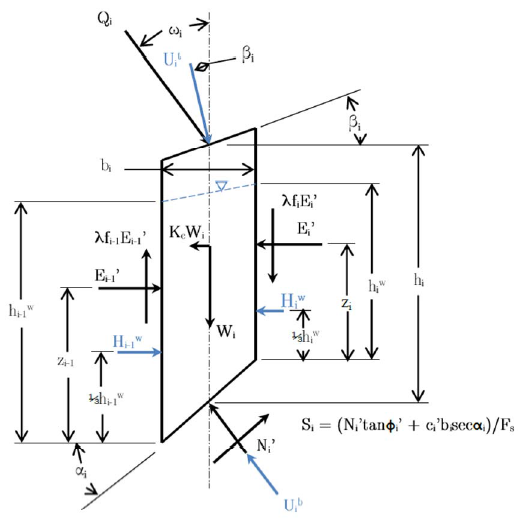
\includegraphics[width=0.4\textwidth]{ForceDiagram.png}
};
\end{tikzpicture}

\begin{tikzpicture}[remember picture,overlay]
\node [xshift=0.5cm,yshift=-2.75cm] at (current page.center)
{
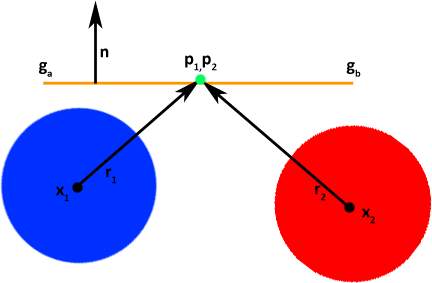
\includegraphics[width=0.3\textwidth]{grooveJoint.png}
};
\end{tikzpicture}

\begin{tikzpicture}[remember picture,overlay]
\node [xshift=4.25cm,yshift=-2.75cm] at (current page.center)
{
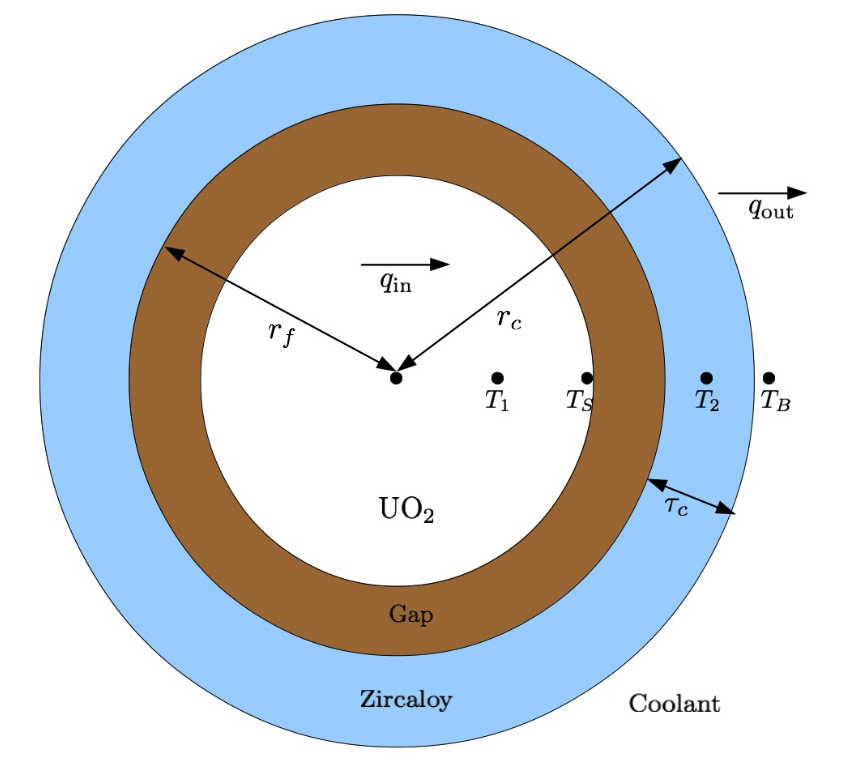
\includegraphics[width=0.3\textwidth]{fuelpin.png}
};
\end{tikzpicture}

\end{frame}
\hoffset=0in

%%%%%%%%%%%%%%%%%%%%%%%%%%%%%%%%%%%%%%

\section[Motivation]{Motivation}

%%%%%%%%%%%%%%%%%%%%%%%%%%%%%%%%%%%%%%

%\hoffset=-.8in
\begin{frame}[plain, fragile]

\frametitle{Motivation: Safety}

% picture of reactor, MRI

\begin{tikzpicture}[remember picture,overlay]
\node [xshift=-0.1cm,yshift=0.75cm] at (current page.center)
{
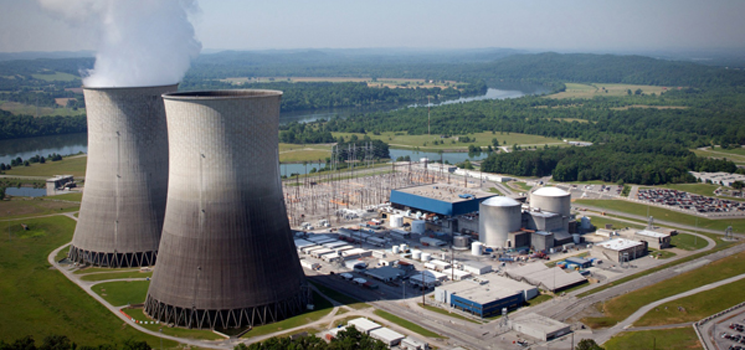
\includegraphics[width=1.1\textwidth]{nuclear_reactor_technologies_home.png}
};
\end{tikzpicture}

\begin{tikzpicture}[remember picture,overlay]
\node [xshift=1.75cm,yshift=-1.75cm] at (current page.center)
{
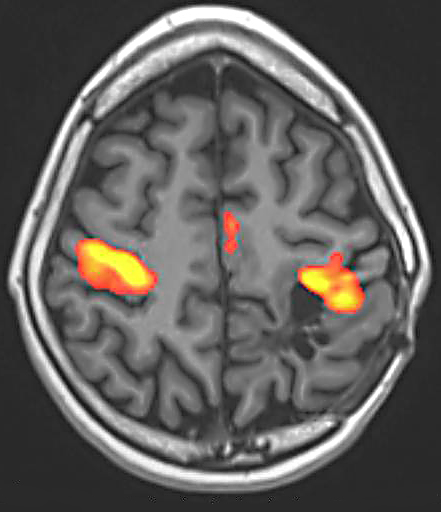
\includegraphics[width=0.4\textwidth]{fmri-image.jpg}
};
\end{tikzpicture}

\end{frame}
\hoffset=0in

%%%%%%%%%%%%%%%%%%%%%%%%%%%%%%%%%%%%%%

%\hoffset=-.8in
\begin{frame}[plain, fragile]

\frametitle{Motivation: (Re)certification}

% picture of stamp

\begin{tikzpicture}[remember picture,overlay]
\node [xshift=0cm,yshift=0cm] at (current page.center)
{

\includegraphics[width=0.8\textwidth]{certified.jpg}
};
\end{tikzpicture}

\end{frame}
\hoffset=0in

%%%%%%%%%%%%%%%%%%%%%%%%%%%%%%%%%%%%%%

\begin{frame}

\frametitle{Motivation: Improve Quality}

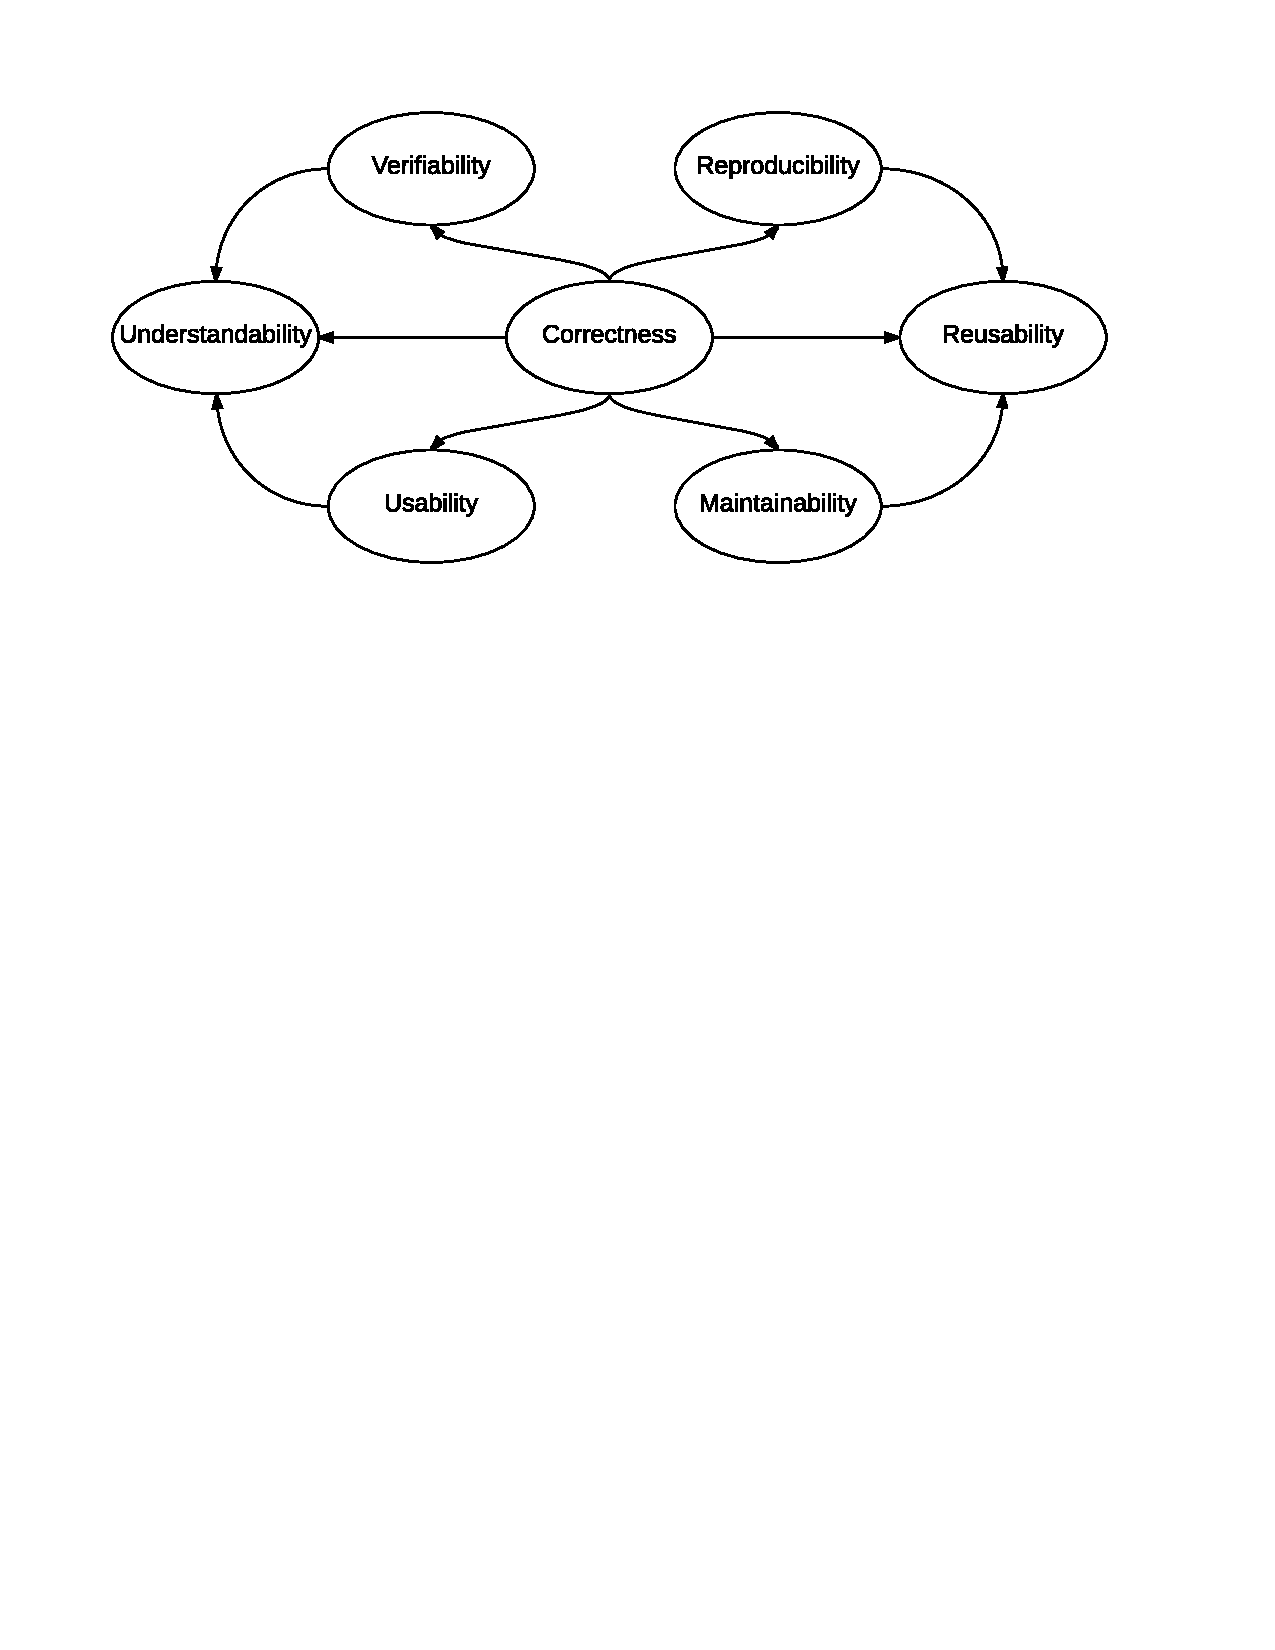
\includegraphics[width=1\textwidth]{RelationBWQualities.pdf}

\end{frame}

%%%%%%%%%%%%%%%%%%%%%%%%%%%%%%%%%%%%%%

% \section[Curr.\ Approach]{Current Approach to Developing SCS}

% %%%%%%%%%%%%%%%%%%%%%%%%%%%%%%%%%%%%%%

% \begin{frame}

% \frametitle{Current Approach}

% \begin{itemize}
% \item Agile like \citep{CarverEtAl2007}
% \item Amethododical \citep{Kelly2013}
% \item Knowledge acquisition driven \citep{Kelly2015}
% \item Each stage reports counterproductive \citep{Roache1998}
% \item Limited tool use \citep{Wilson2006}
% \item Limited testing of code \citep{KellyAndSanders2008a}
% \item Lack of understanding of testing \citep{Merali2010}
% \item Missed opportunities for reuse \citep{Owen1998} 
%  %-- 37 of 52 triangular mesh generators
%  % implemented the same triangulation algorithm
% \item Emphasis on:
% \begin{enumerate}
% \item Science~\citep{Kelly2007}
% \item Code
% \end{enumerate}
% \end{itemize}

% \end{frame}

% %%%%%%%%%%%%%%%%%%%%%%%%%%%%%%%%%%%%%%

% \begin{frame}

% \frametitle{Challenges for DDD}

% \begin{itemize}
% \item Up front requirements
% \item Rapid change for numerical algorithms
% \item Information duplication
% \item Synchronization headaches between artifacts
% \item Perceived over-emphasis on non-executable artifacts
% %Parnas paper - people do not like docs, vicious cycle
% \end{itemize}

% \end{frame}

%%%%%%%%%%%%%%%%%%%%%%%%%%%%%%%%%%%%%%

\section[DDD]{Document Driven Design}

%%%%%%%%%%%%%%%%%%%%%%%%%%%%%%%%%%%%%%

\begin{frame}

\frametitle{``Faked'' Rational Design Process}

\begin{center}
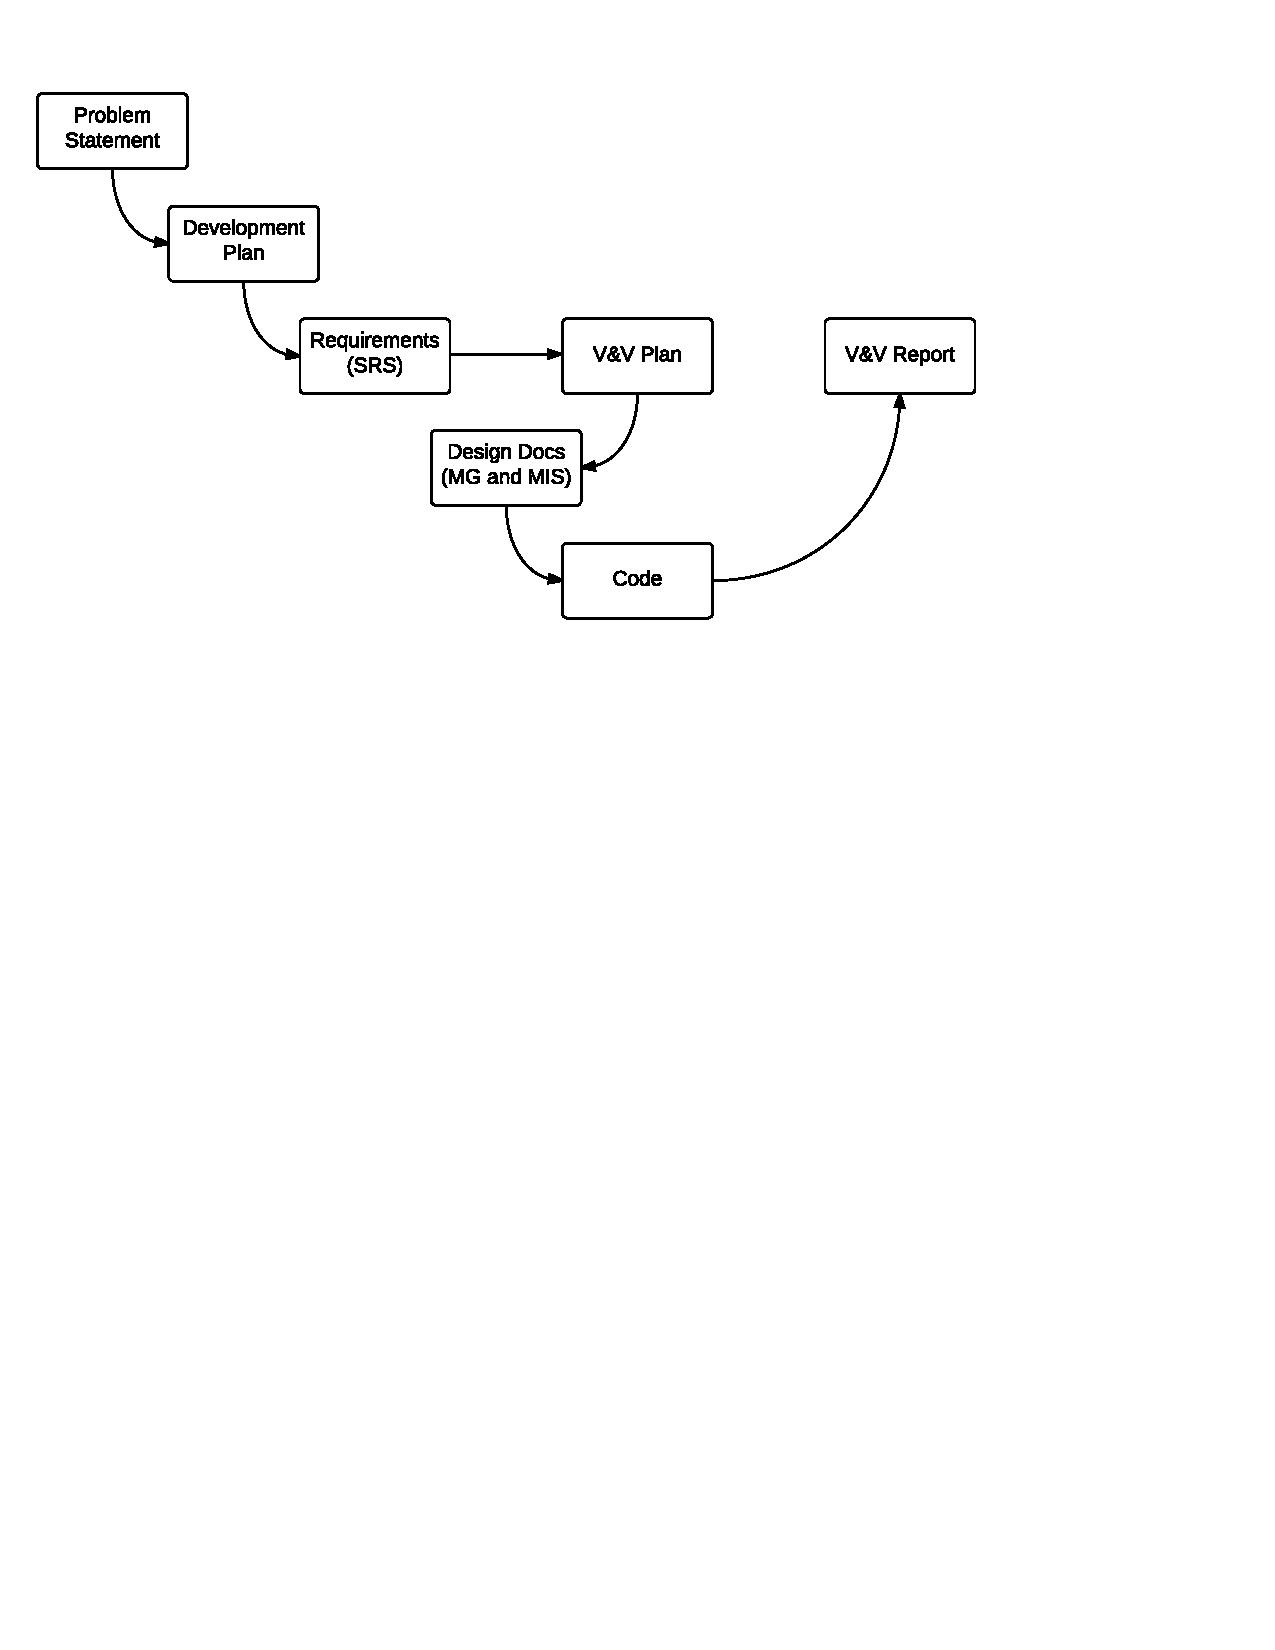
\includegraphics[scale=0.6]{OverviewOfProcess.pdf}
\end{center}

SWHS example at
\href{https://github.com/smiths/swhs}{https://github.com/smiths/swhs}

\end{frame}

%%%%%%%%%%%%%%%%%%%%%%%%%%%%%%%%%%%%%%

\begin{frame}

\frametitle{The Challenge}

\begin{itemize}
\item Documentation provides advantages
\begin{itemize}
\item Improves verifiability, reusability, reproducibility, etc.
\item From \cite{Parnas2010}
\begin{itemize}
\item easier reuse of old designs
\item better communication about requirements
\item more
  useful design reviews
\item etc.
% \item easier integration of separately written modules, more
%   effective code inspection, more effective testing, and more efficient
%   corrections and improvements
\end{itemize}
\item New doc found 27 errors \citep{SmithAndKoothoor2016}
\item Developers see advantage \citep{SmithJegatheesanAndKelly2016}
\end{itemize}
\item But documentation is felt to be ...
\begin{itemize}
\item Too long
\item Too difficult to maintain
\item Not amenable to change
\item Too tied to waterfall process
\item Reports counterproductive \citep{Roache1998}
\end{itemize}
\item \structure{\textbf{The Solution?}}
\end{itemize}

\end{frame}

%%%%%%%%%%%%%%%%%%%%%%%%%%%%%%%%%%%%%%

\section[Drasil]{Drasil}

%%%%%%%%%%%%%%%%%%%%%%%%%%%%%%%%%%%%%%

\subsection[Overview]{Overview of Drasil}

%%%%%%%%%%%%%%%%%%%%%%%%%%%%%%%%%%%%%%

\begin{frame}

\includegraphics[width=1\textwidth]{../WG2_11/generate_all_the_things.jpg}
\end{frame}

%%%%%%%%%%%%%%%%%%%%%%%%%%%%%%%%%%%%%%

\begin{frame}

\frametitle{Knowledge Capture}

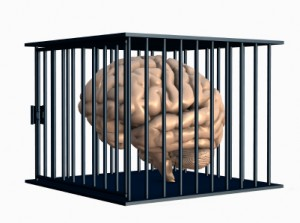
\includegraphics[width=1.0\textwidth]{KC.jpg}

\end{frame}

%%%%%%%%%%%%%%%%%%%%%%%%%%%%%%%%%%%%%%

\begin{frame}

\frametitle{Drasil}
\begin{center}
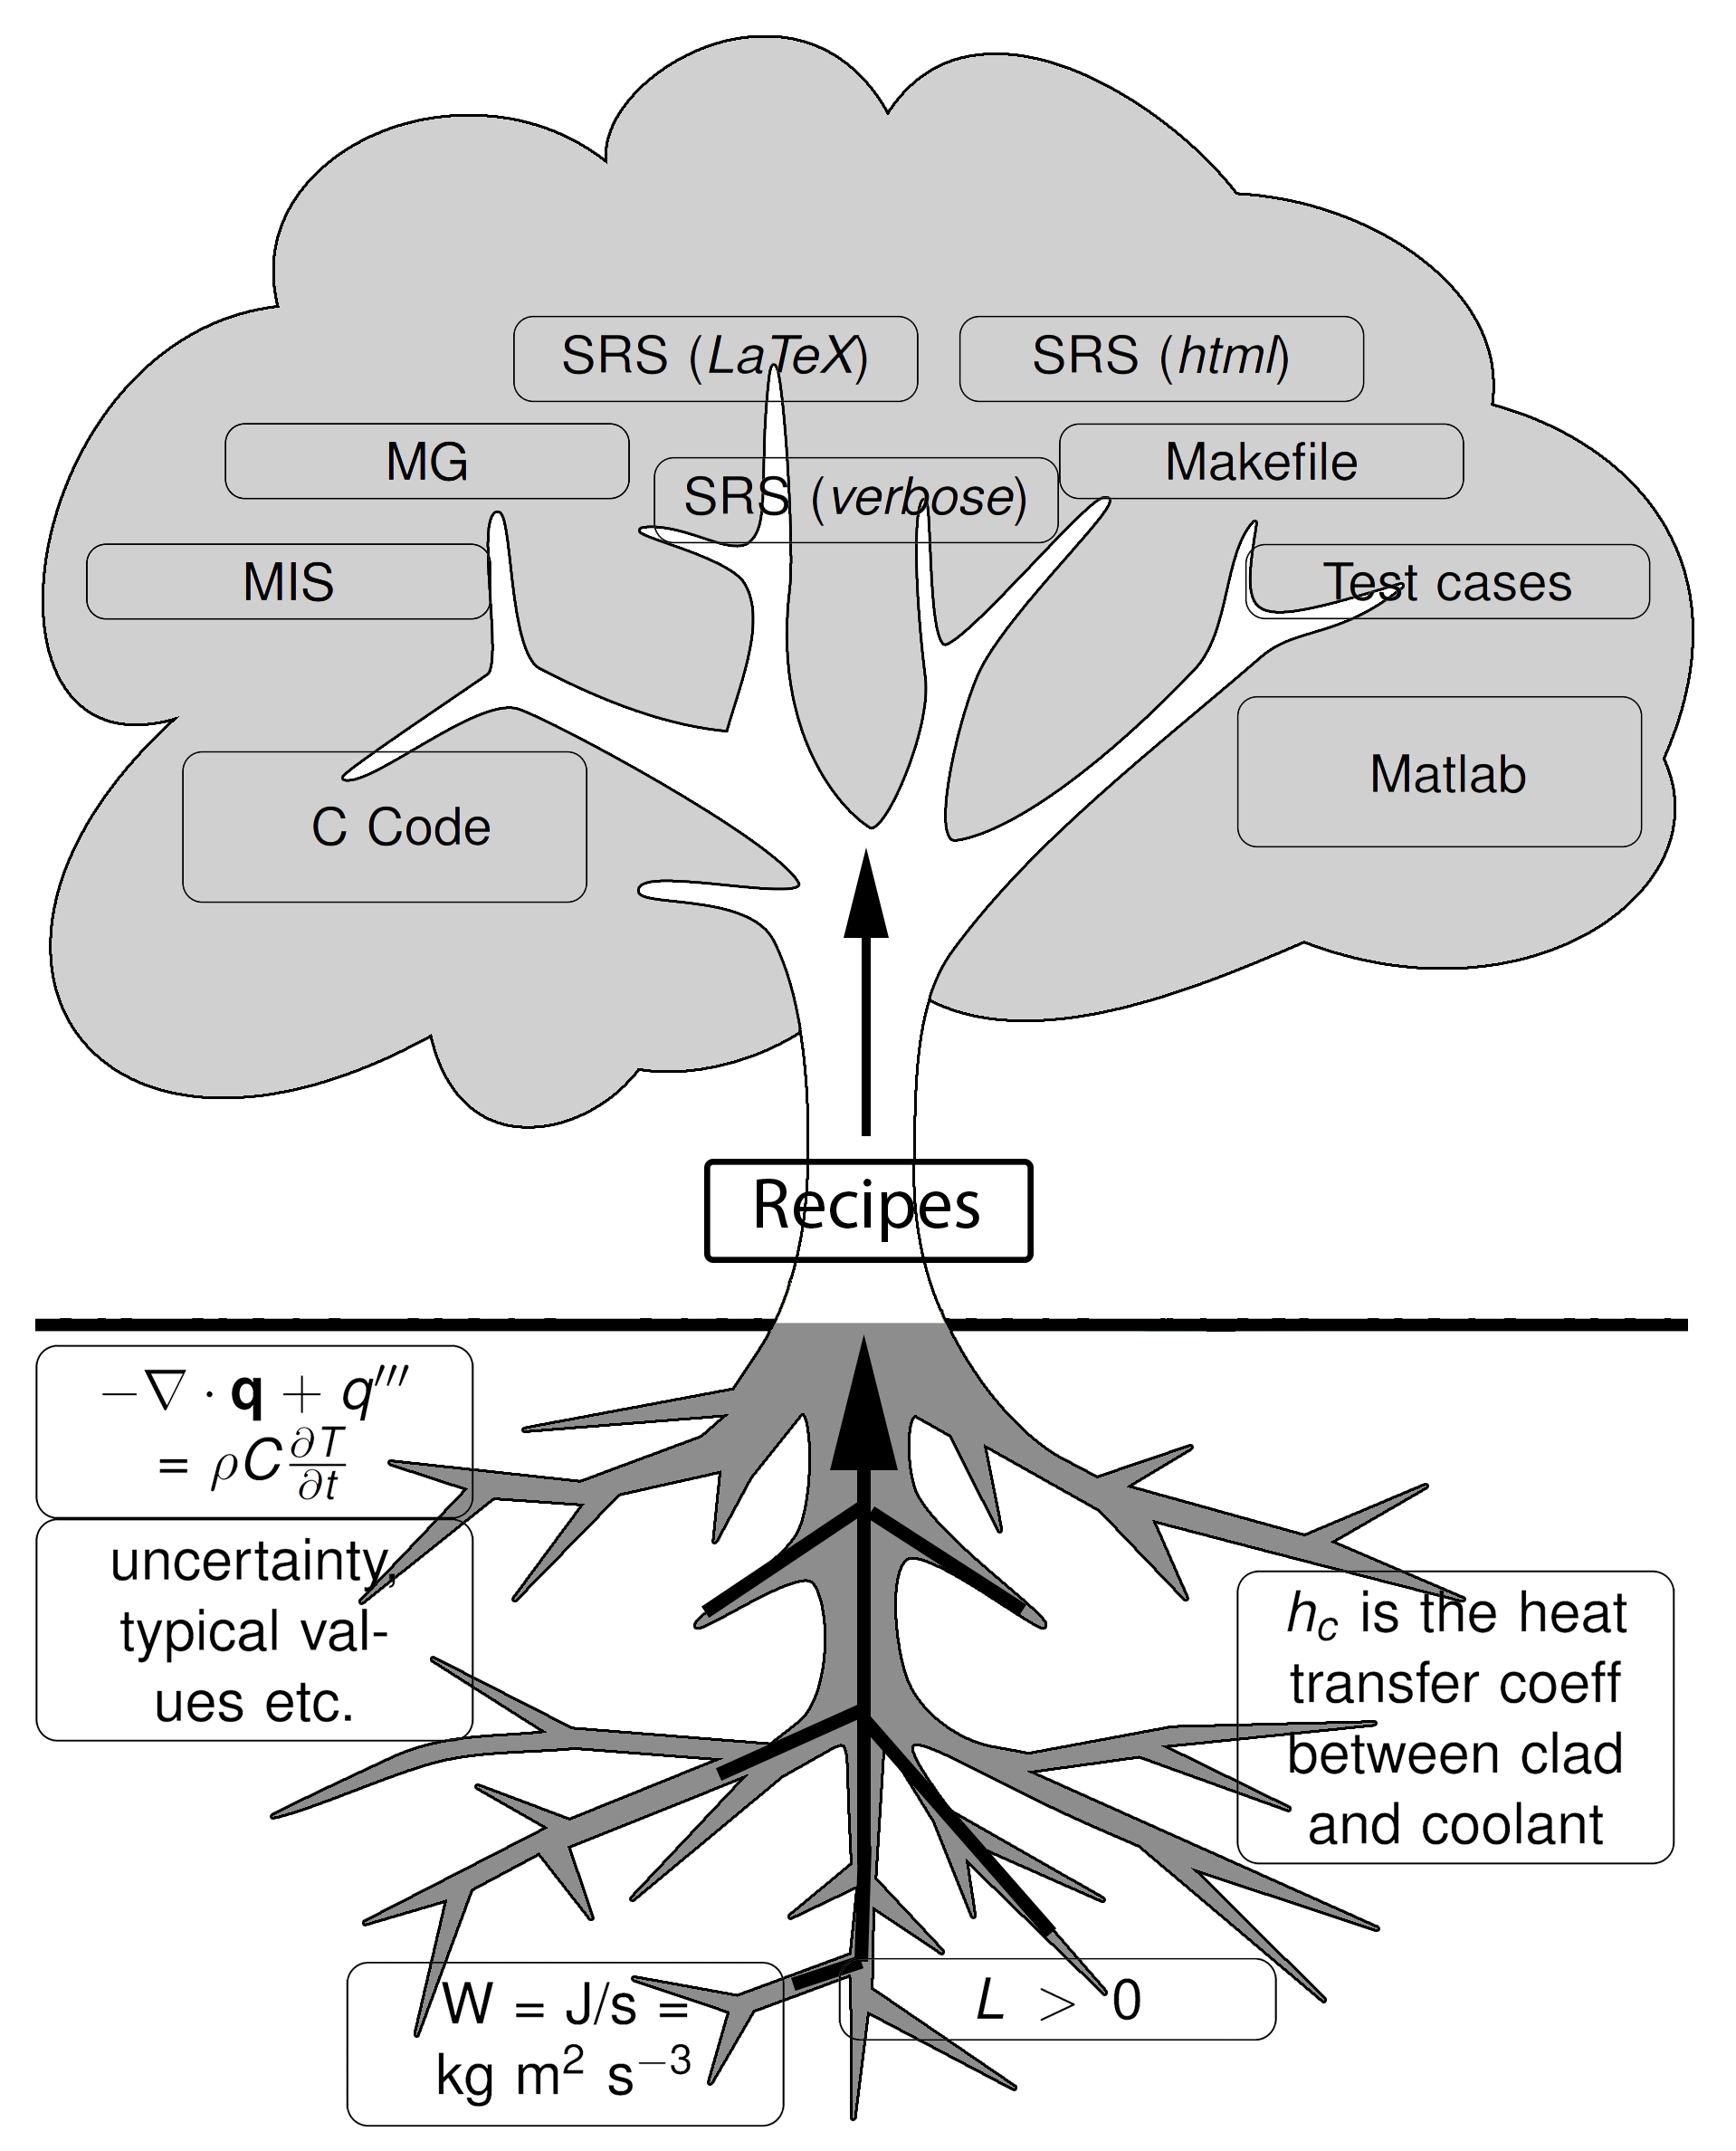
\includegraphics[height=21em]{tree.png}
\end{center}
\end{frame}

%%%%%%%%%%%%%%%%%%%%%%%%%%%%%%%%%%%%%

\begin{frame}
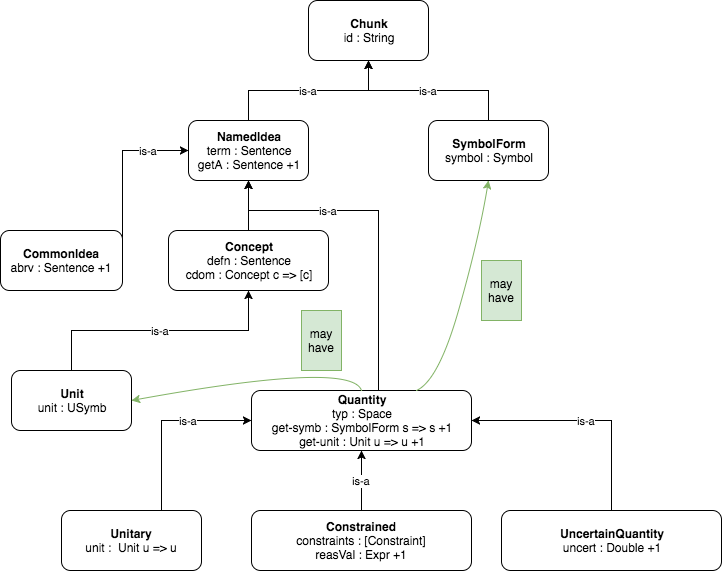
\includegraphics[width=1\textwidth]{class_hierarchy.png}
\end{frame}

%%%%%%%%%%%%%%%%%%%%%%%%%%%%%%%%%%%%%

% \begin{frame}

% \frametitle{Knowledge Based Approach}

% \begin{itemize}
% \item Capture knowledge
% \item From one ``source'' recipes to generate artifacts
% \item Automated
% \item Inspired by Knuth's Literate Programming
% \end{itemize}
% \end{frame}

%%%%%%%%%%%%%%%%%%%%%%%%%%%%%%%%%%%%%%

\subsection[Example]{Example}

%%%%%%%%%%%%%%%%%%%%%%%%%%%%%%%%%%%%%%

\begin{frame}

\frametitle{$J_{\mbox{tol}}$ in SRS.pdf}
\begin{center}
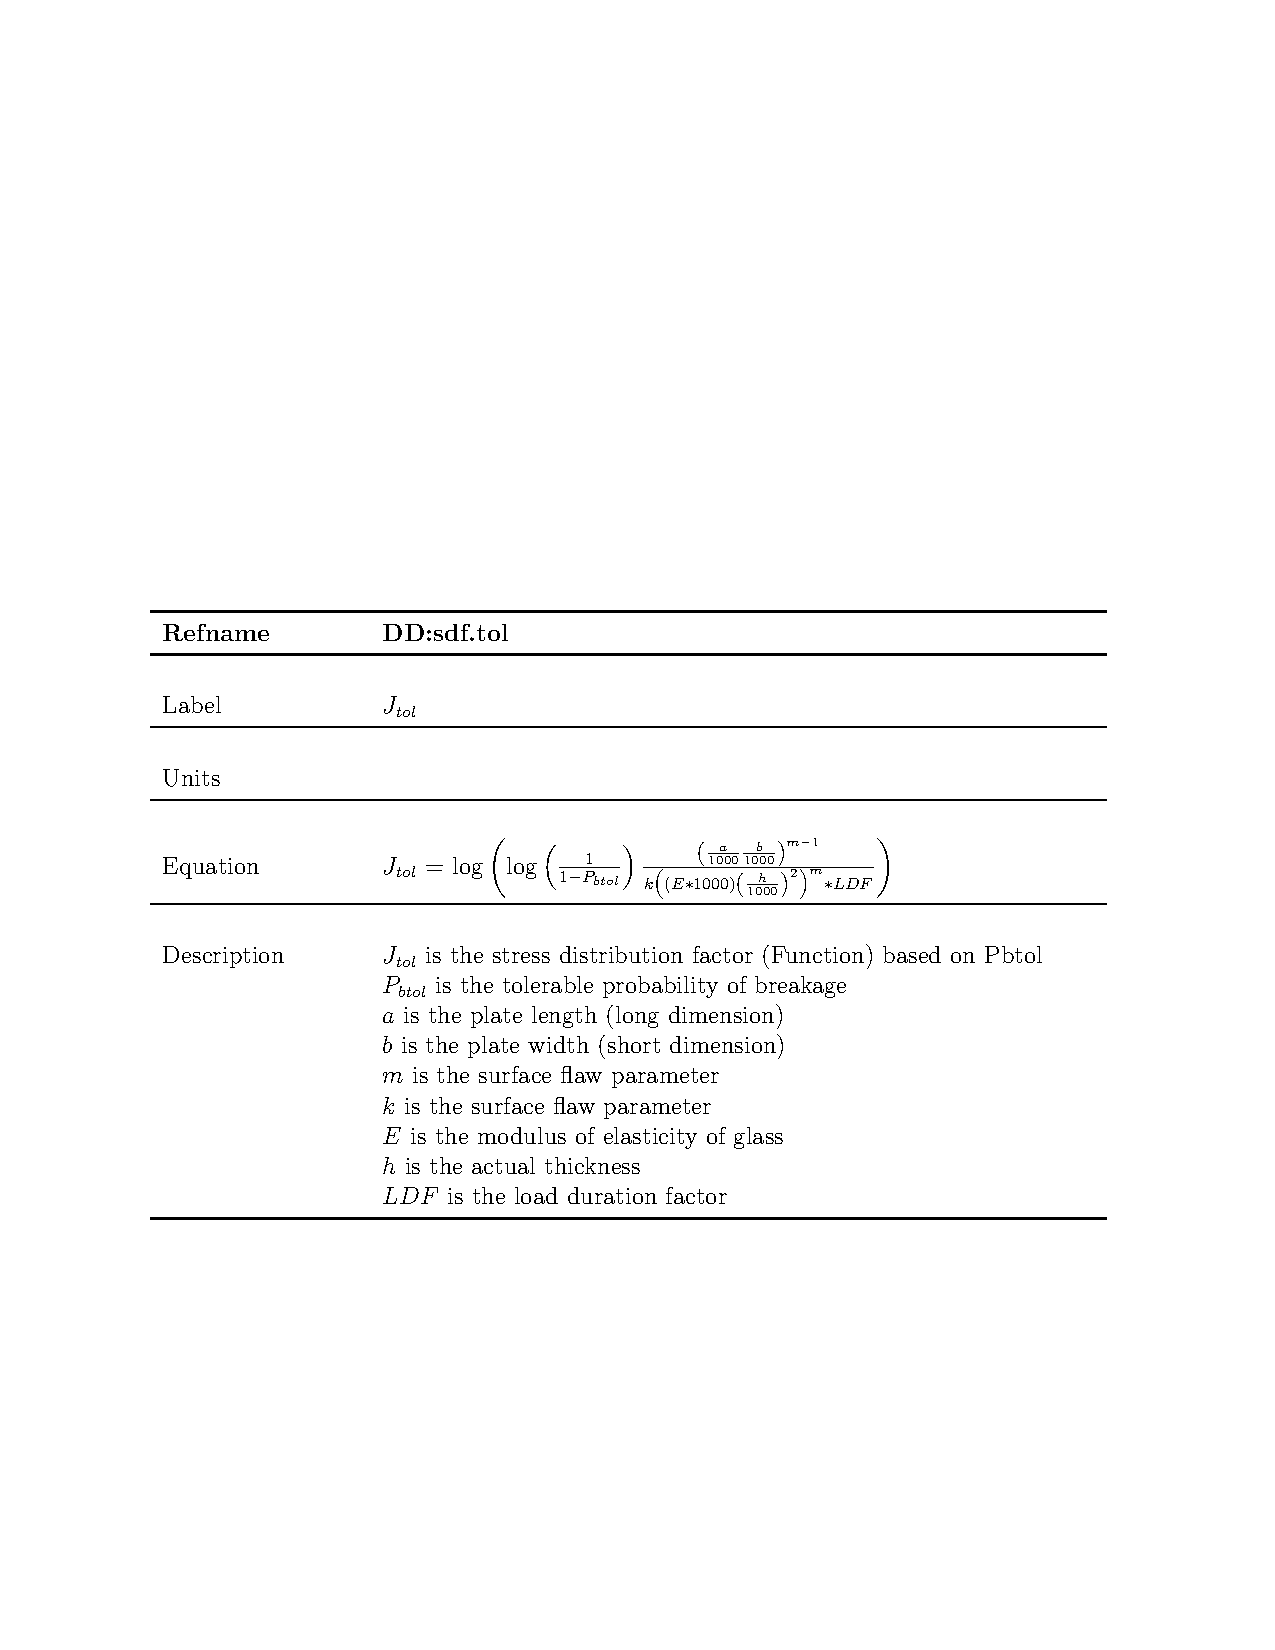
\includegraphics[width=1.0\textwidth]{Jtol_pdf.pdf}
\end{center}
\end{frame}

%%%%%%%%%%%%%%%%%%%%%%%%%%%%%%%%%%%%%

\begin{frame}[plain, fragile]

\frametitle{$J_{\mbox{tol}}$ in SRS.tex}
~\\
\begin{lstlisting}
\noindent \begin{minipage}{\textwidth}
\begin{tabular}{p{0.2\textwidth} p{0.73\textwidth}}
\toprule \textbf{Refname} & \textbf{DD:sdf.tol}
\phantomsection 
\label{DD:sdf.tol}
\\ \midrule \\
Label & $J_{tol}$
\\ \midrule \\
Units & 
\\ \midrule \\
Equation & $J_{tol}$ = $\log\left(\log\left(\frac{1}{1-P_{btol}}\right)\frac{\left(\frac{a}{1000}\frac{b}{1000}\right)^{m-1}}{k\left(\left(E*1000\right)\left(\frac{h}{1000}\right)^{2}\right)^{m}*LDF}\right)$
\\ \midrule \\
Description & $J_{tol}$ is the stress distribution factor (Function) based on
              Pbtol\newline$P_{btol}$ is the tolerable probability of breakage ...
\end{minipage}\\
\end{lstlisting}
\end{frame}

%%%%%%%%%%%%%%%%%%%%%%%%%%%%%%%%%%%%%%

\begin{frame}[plain, fragile]

\frametitle{$J_{\mbox{tol}}$ in SRS.html}

\begin{lstlisting}

<a id="">
<div class="equation">
<em>J<sub>tol</sub></em> = log(log(<div class="fraction">
<span class="fup">
1
</span>
<span class="fdn">
1 &minus; <em>P<sub>btol</sub></em>
</span>
</div>)<div class="fraction">
<span class="fup">
(<div class="fraction">
<span class="fup">
<em>a</em>
</span>
<span class="fdn">
1000
</span>
</div><div class="fraction">
...
\end{lstlisting}

\end{frame}
%%%%%%%%%%%%%%%%%%%%%%%%%%%%%%%%%%%%%

\begin{frame}[plain, fragile]

\frametitle{$J_{\mbox{tol}}$ in Python}

\begin{lstlisting}
def calc_j_tol(inparams):
    j_tol = math.log((math.log(1.0 / (1.0 - inparams.pbtol))) * ((((inparams.a / 1000.0) * (inparams.b / 1000.0)) ** (inparams.m - 1.0)) / ((inparams.k * (((inparams.E * 1000.0) * ((inparams.h / 1000.0) ** 2.0)) ** inparams.m)) * inparams.ldf)))
    return j_tol
\end{lstlisting}
\end{frame}

%%%%%%%%%%%%%%%%%%%%%%%%%%%%%%%%%%%%%%

\begin{frame}[plain, fragile]

\frametitle{$J_{\mbox{tol}}$ in Java}

\begin{lstlisting}
public static double calc_j_tol(InputParameters inparams) {
        double j_tol = Math.log((Math.log(1.0 / (1.0 - inparams.pbtol))) * ((Math.pow((inparams.a / 1000.0) * (inparams.b / 1000.0), inparams.m - 1.0)) / ((inparams.k * (Math.pow((inparams.E * 1000.0) * (Math.pow(inparams.h / 1000.0, 2.0)), inparams.m))) * inparams.ldf)));
        return j_tol;
    }
\end{lstlisting}
\end{frame}

%%%%%%%%%%%%%%%%%%%%%%%%%%%%%%%%%%%%%%

\begin{frame}[plain, fragile]

\frametitle{$J_{\mbox{tol}}$ in Drasil (Haskell)}

\begin{lstlisting}
stressDistFac = makeVC "stressDistFac" (nounPhraseSP 
  $ "stress distribution" ++ " factor (Function)") cJ

sdf_tol = makeVC "sdf_tol" (nounPhraseSP $ 
  "stress distribution" ++
  " factor (Function) based on Pbtol") 
  (sub (stressDistFac ^. symbol) (Atomic "tol"))

tolStrDisFac_eq :: Expr
tolStrDisFac_eq = log (log ((1) / ((1) - (C pb_tol)))
  * ((Grouping (((C plate_len) / (1000)) * ((C plate_width) / (1000)))) :^
  ((C sflawParamM) - (1)) / ((C sflawParamK) *
  (Grouping (Grouping ((C mod_elas) * (1000)) *
  (square (Grouping ((C act_thick) / (1000))))
  )) :^ (C sflawParamM) * (C loadDF))))

tolStrDisFac :: QDefinition
tolStrDisFac = mkDataDef sdf_tol tolStrDisFac_eq
\end{lstlisting}
\end{frame}

%%%%%%%%%%%%%%%%%%%%%%%%%%%%%%%%%%%%%%

\begin{frame}[plain, fragile]

\frametitle{$J_{\mbox{tol}}$ without Unit Conversion}

\begin{lstlisting}
tolStrDisFac_eq :: Expr
tolStrDisFac_eq = log (log ((1) / ((1) - (C pb_tol)))
  * ((Grouping ((C plate_len) * (C plate_width))) :^
  ((C sflawParamM) - (1)) / ((C sflawParamK) *
  (Grouping ((C mod_elas) * (square (C act_thick)))) :^ (C sflawParamM) * (C loadDF))))
\end{lstlisting}
\end{frame}

%%%%%%%%%%%%%%%%%%%%%%%%%%%%%%%%%%%%%%

\subsection[SRS]{SRS}

%%%%%%%%%%%%%%%%%%%%%%%%%%%%%%%%%%%%%%

\hoffset=-.4in %removing side bar for these frames

\begin{frame}[plain, fragile]

%\frametitle{SRS for SWHS}

\begin{center}
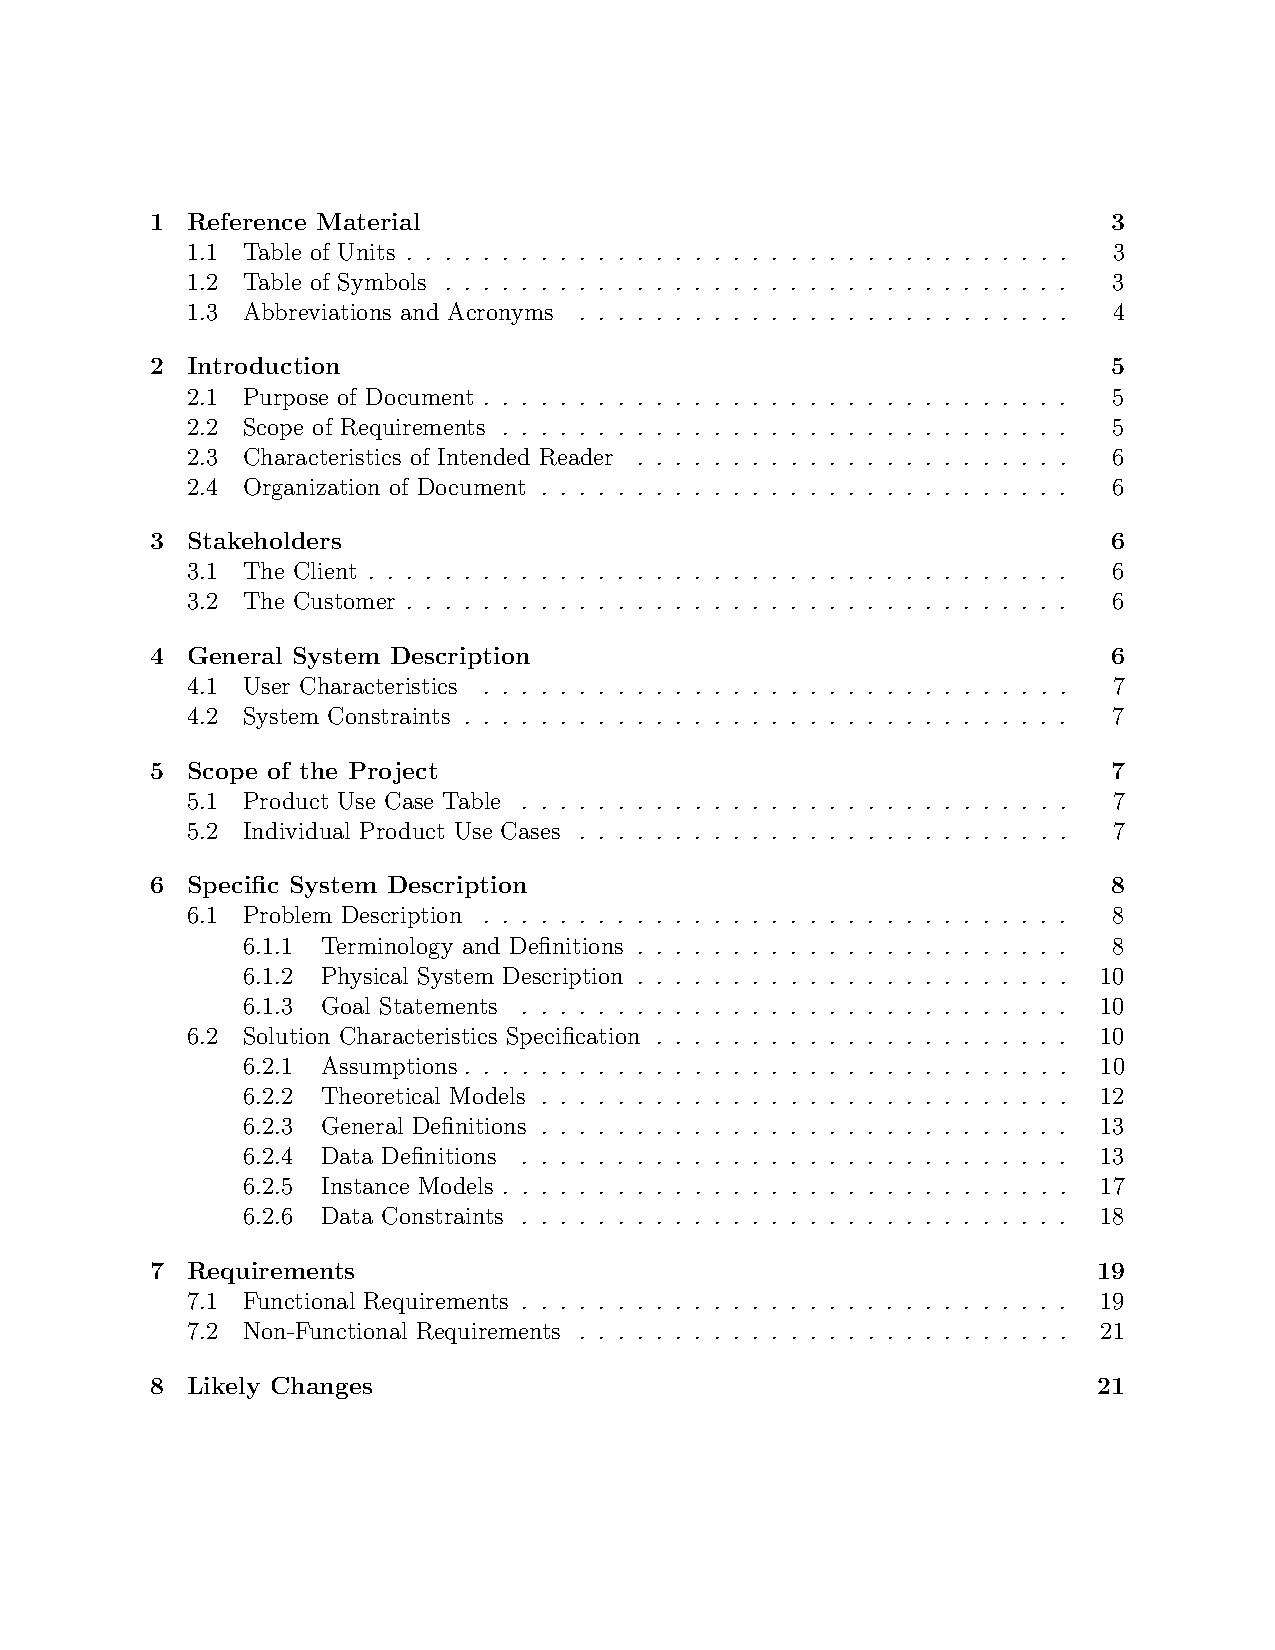
\includegraphics[scale=0.45]{TofC.pdf}
\end{center}

\end{frame}
\hoffset=0in

%%%%%%%%%%%%%%%%%%%%%%%%%%%%%%%%%%%%%%

\hoffset=-.7in %removing side bar for these frames

\begin{frame}[plain, fragile]

\frametitle{Traceability Graph}

\begin{center}
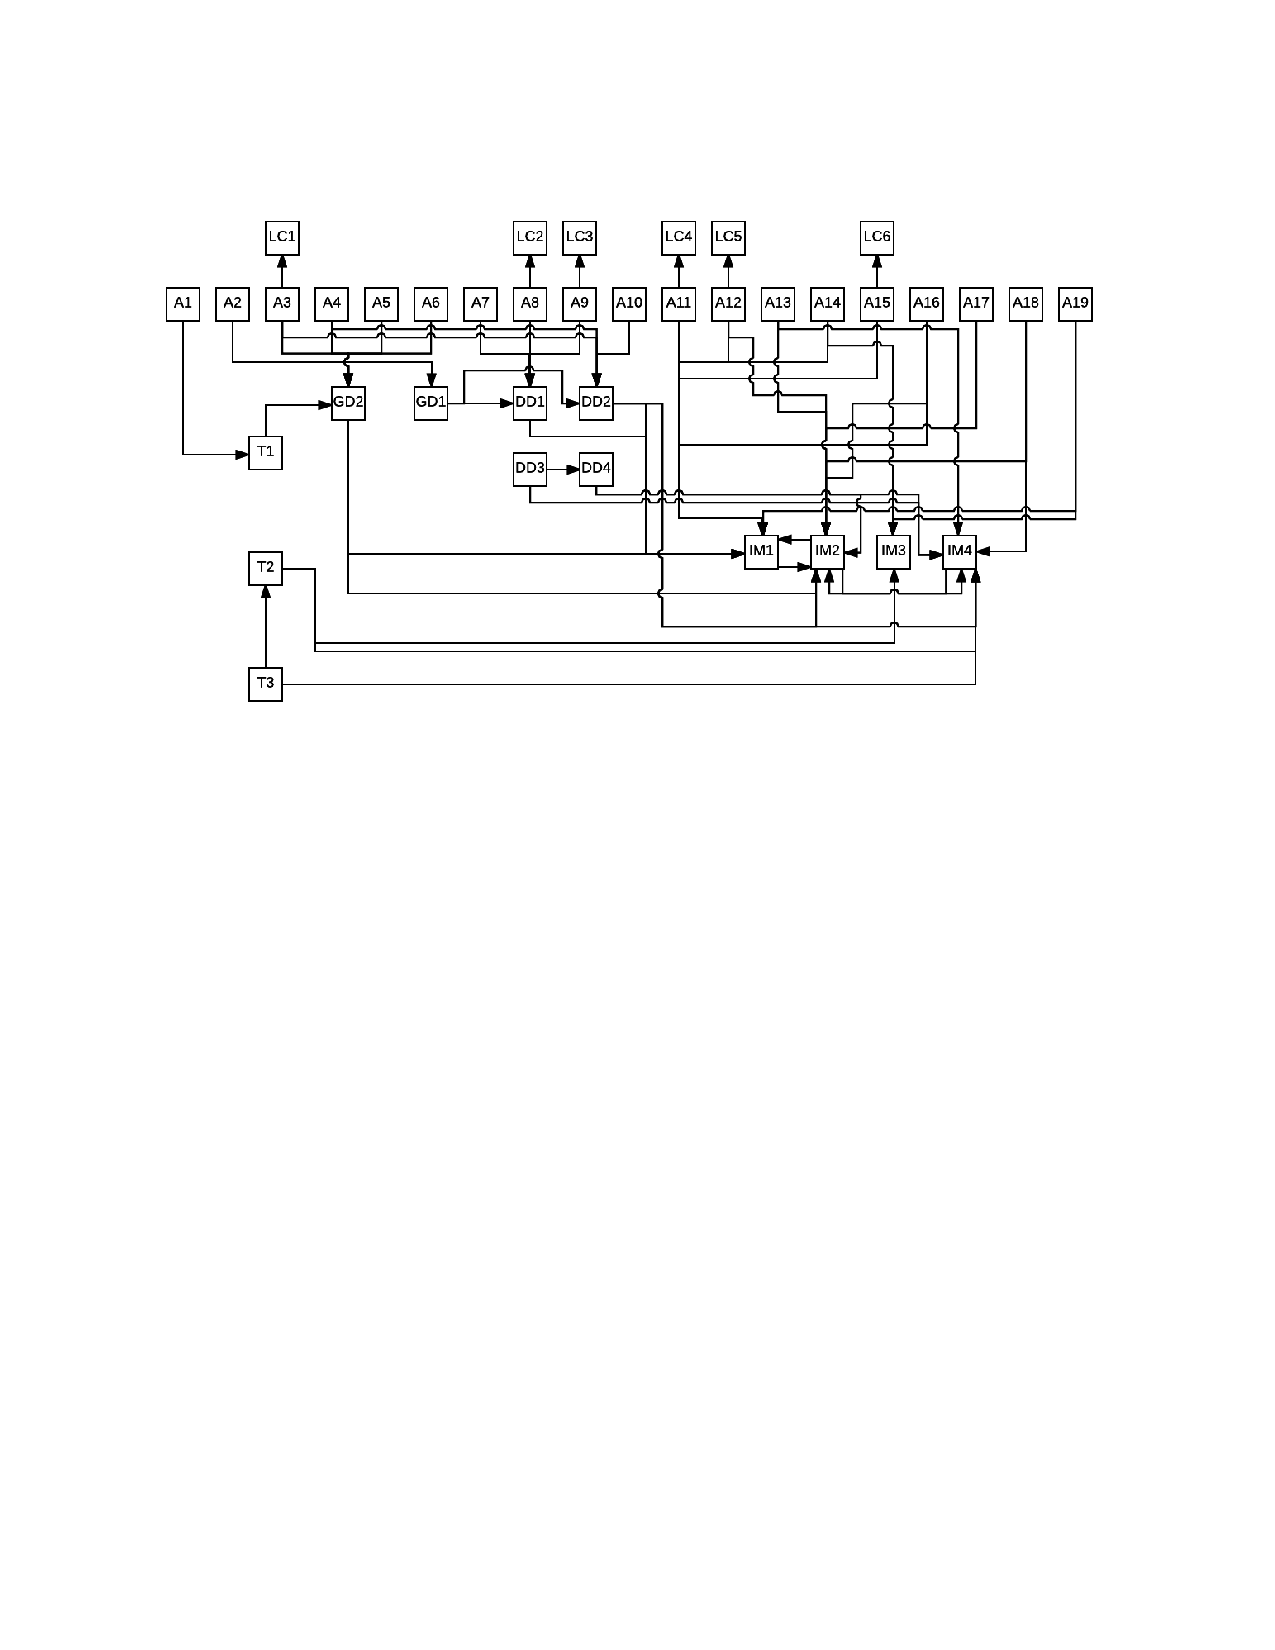
\includegraphics[scale=0.75]{TraceGraph.pdf}
\end{center}

\end{frame}
\hoffset=0in

%%%%%%%%%%%%%%%%%%%%%%%%%%%%%%%%%%%%%%

\section[Qualities]{Qualities}

%%%%%%%%%%%%%%%%%%%%%%%%%%%%%%%%%%%%%%

\begin{frame}

\frametitle{Verifiability}

\begin{table} 
\centering
%\caption{Constraints on quantities}
\begin{tabular}{c c r c } 
\toprule
\textbf{Var} & \textbf{Constraints} & \textbf{Typical Value} & \textbf{Uncertainty}\\ \midrule
$L$ & $L > 0$ & 1.5 m & 10\% \\ 
$\rho_P$ & $\rho_P > 0$	& 1007 kg/m$^3$	& 10\% \\
\bottomrule
\end{tabular}
\label{tab:pcm}
\end{table}

\begin{equation*}
E_W = \int_{0}^{t} h_C A_C (T_C - T_W(t)) dt - \int_{0}^{t} h_P A_P (T_W(t) - T_P(t)) dt
\end{equation*}

\begin{itemize}
\item If wrong, wrong everywhere
\item Sanity checks captured and reused
\item Generate guards against invalid input
\item Generate test cases
\item Generate view suitable for inspection
\item Traceability
\end{itemize}
\end{frame}

%%%%%%%%%%%%%%%%%%%%%%%%%%%%%%%%%%%%%%

\begin{frame}

\frametitle{Reusability}

\begin{itemize}
\item De-embed knowledge
\item Reuse throughout document
\begin{itemize}
\item Units
\item Symbols
\item Descriptions
\item Traceability information
\end{itemize}
\item Reuse between documents
\begin{itemize}
\item SRS
\item MIS
\item Code
\item Test cases
\end{itemize}
\item Reuse between projects
\begin{itemize}
\item Knowledge reuse
\item For a family of related models or reuses of portions of knowledge
\item Conservation of thermal energy
\item Interpolation
\item Etc.
\end{itemize}
\end{itemize}
\end{frame}

%%%%%%%%%%%%%%%%%%%%%%%%%%%%%%%%%%%%%%

\begin{frame}

\frametitle{Reproducibility}

\begin{itemize}
\item Usual emphasis is on reproducing code execution
\item However, \cite{IonescuAndJansson2013} show reproducibility challenges due to
undocumented:
\begin{itemize}
\item Assumptions
\item Modifications
\item Hacks
\end{itemize}
\item Shouldn't it be easier to independently replicate the work of others?
\item Require theory, assumptions, equations, etc.
\item Drasil can potentially check for completeness and consistency
\end{itemize}

\end{frame}

%%%%%%%%%%%%%%%%%%%%%%%%%%%%%%%%%%%%%%

\section[Future Work]{Future Work}

%%%%%%%%%%%%%%%%%%%%%%%%%%%%%%%%%%%%%%

\begin{frame}

\includegraphics[width=\textwidth]{no_silver_bullet.jpg}
\end{frame}

%%%%%%%%%%%%%%%%%%%%%%%%%%%%%%%%%%%%%
\hoffset=-.7in %removing side bar for these frames
\begin{frame}[plain]

\frametitle{Future Work}

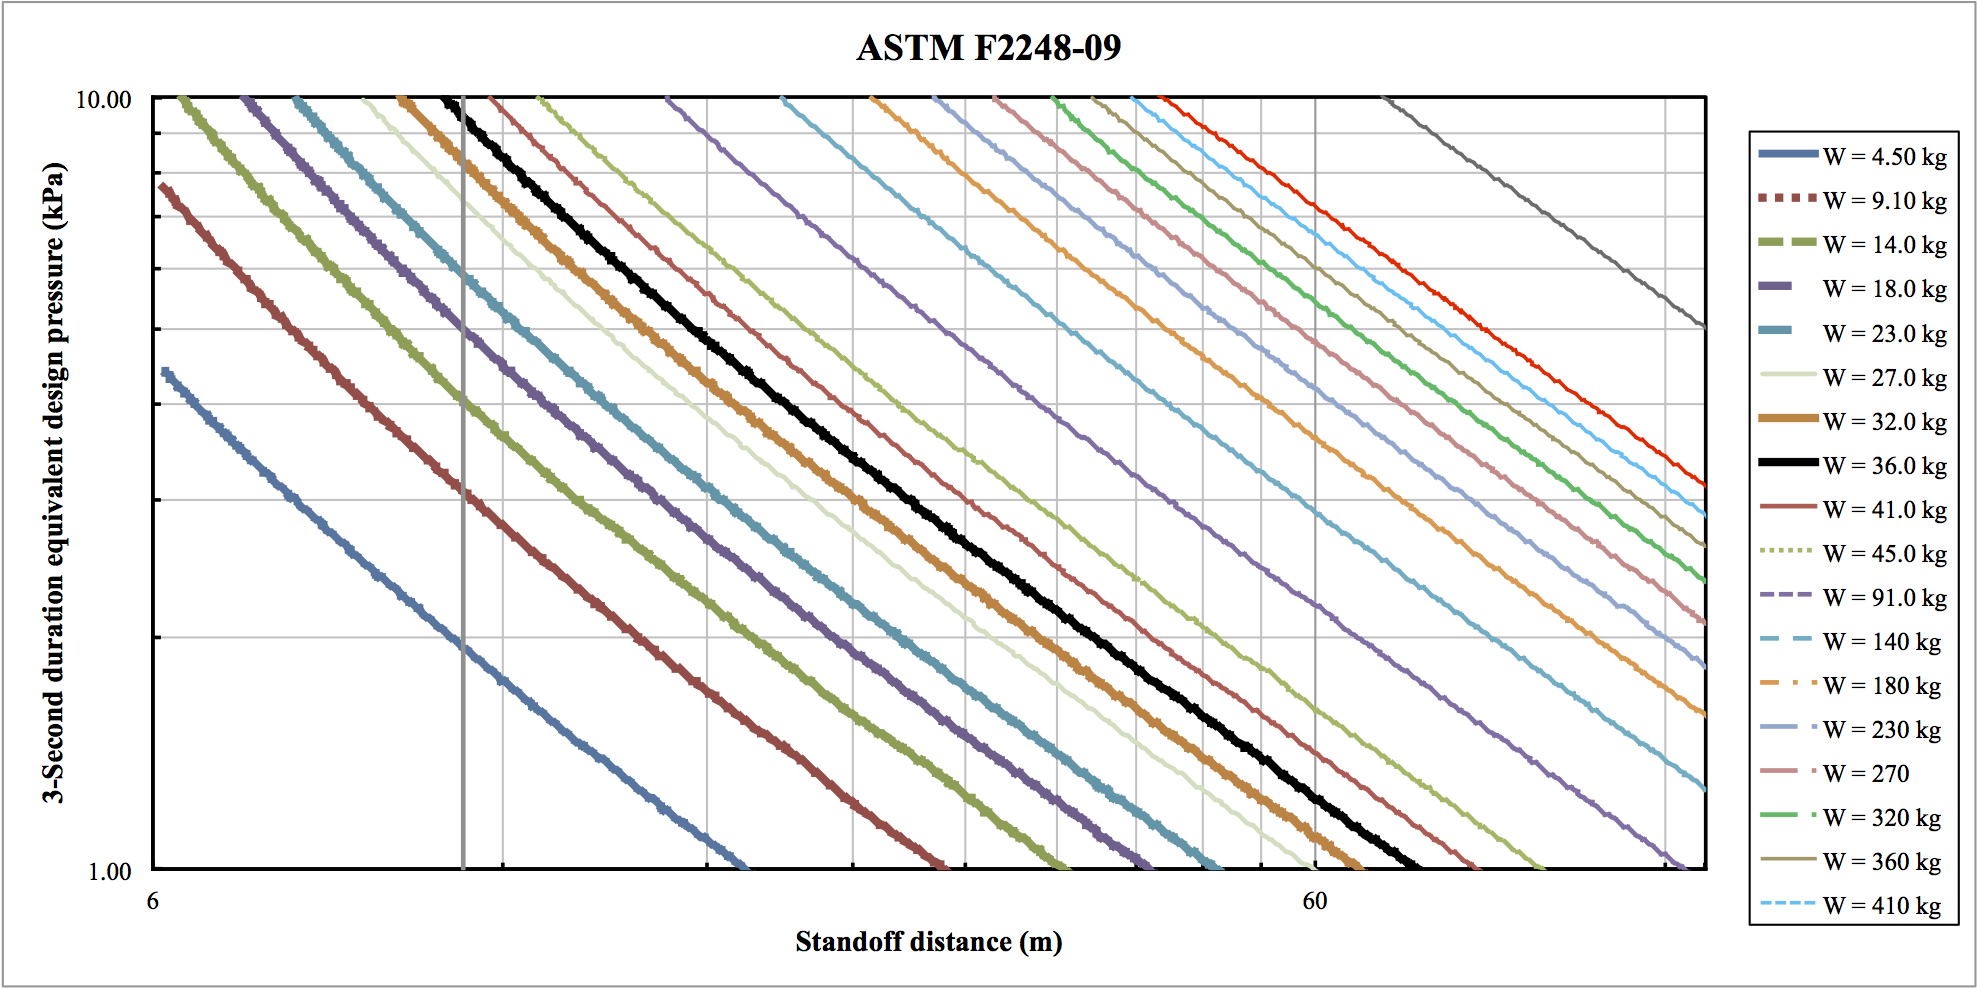
\includegraphics[width=1.2\textwidth]{ASTM_F2248-09.png}

\end{frame}
\hoffset=0in %reset side bar for these frames
%%%%%%%%%%%%%%%%%%%%%%%%%%%%%%%%%%%%%%

\section[Conclusions]{Conclusions}

%%%%%%%%%%%%%%%%%%%%%%%%%%%%%%%%%%%%%%

\begin{frame}

\frametitle{Drasil Framework for LSS}

\begin{itemize}
\item SCS has the opportunity to lead other software fields%  by leveraging its
  % solid existing knowledge base
\item Document driven design is feasible% with a knowledge-based approach
\item Requires an investment of time %to build knowledge base
\item Documentation does not have to be painful
\item Develop/refactor via practical case studies
\item Ontology may naturally emerge
\end{itemize}


\includegraphics[width=0.5\textwidth]{../WG2_11/generate_all_the_things.jpg}

\begin{tikzpicture}[remember picture,overlay]
\node [xshift=2.75cm,yshift=-2.15cm] at (current page.center)
{
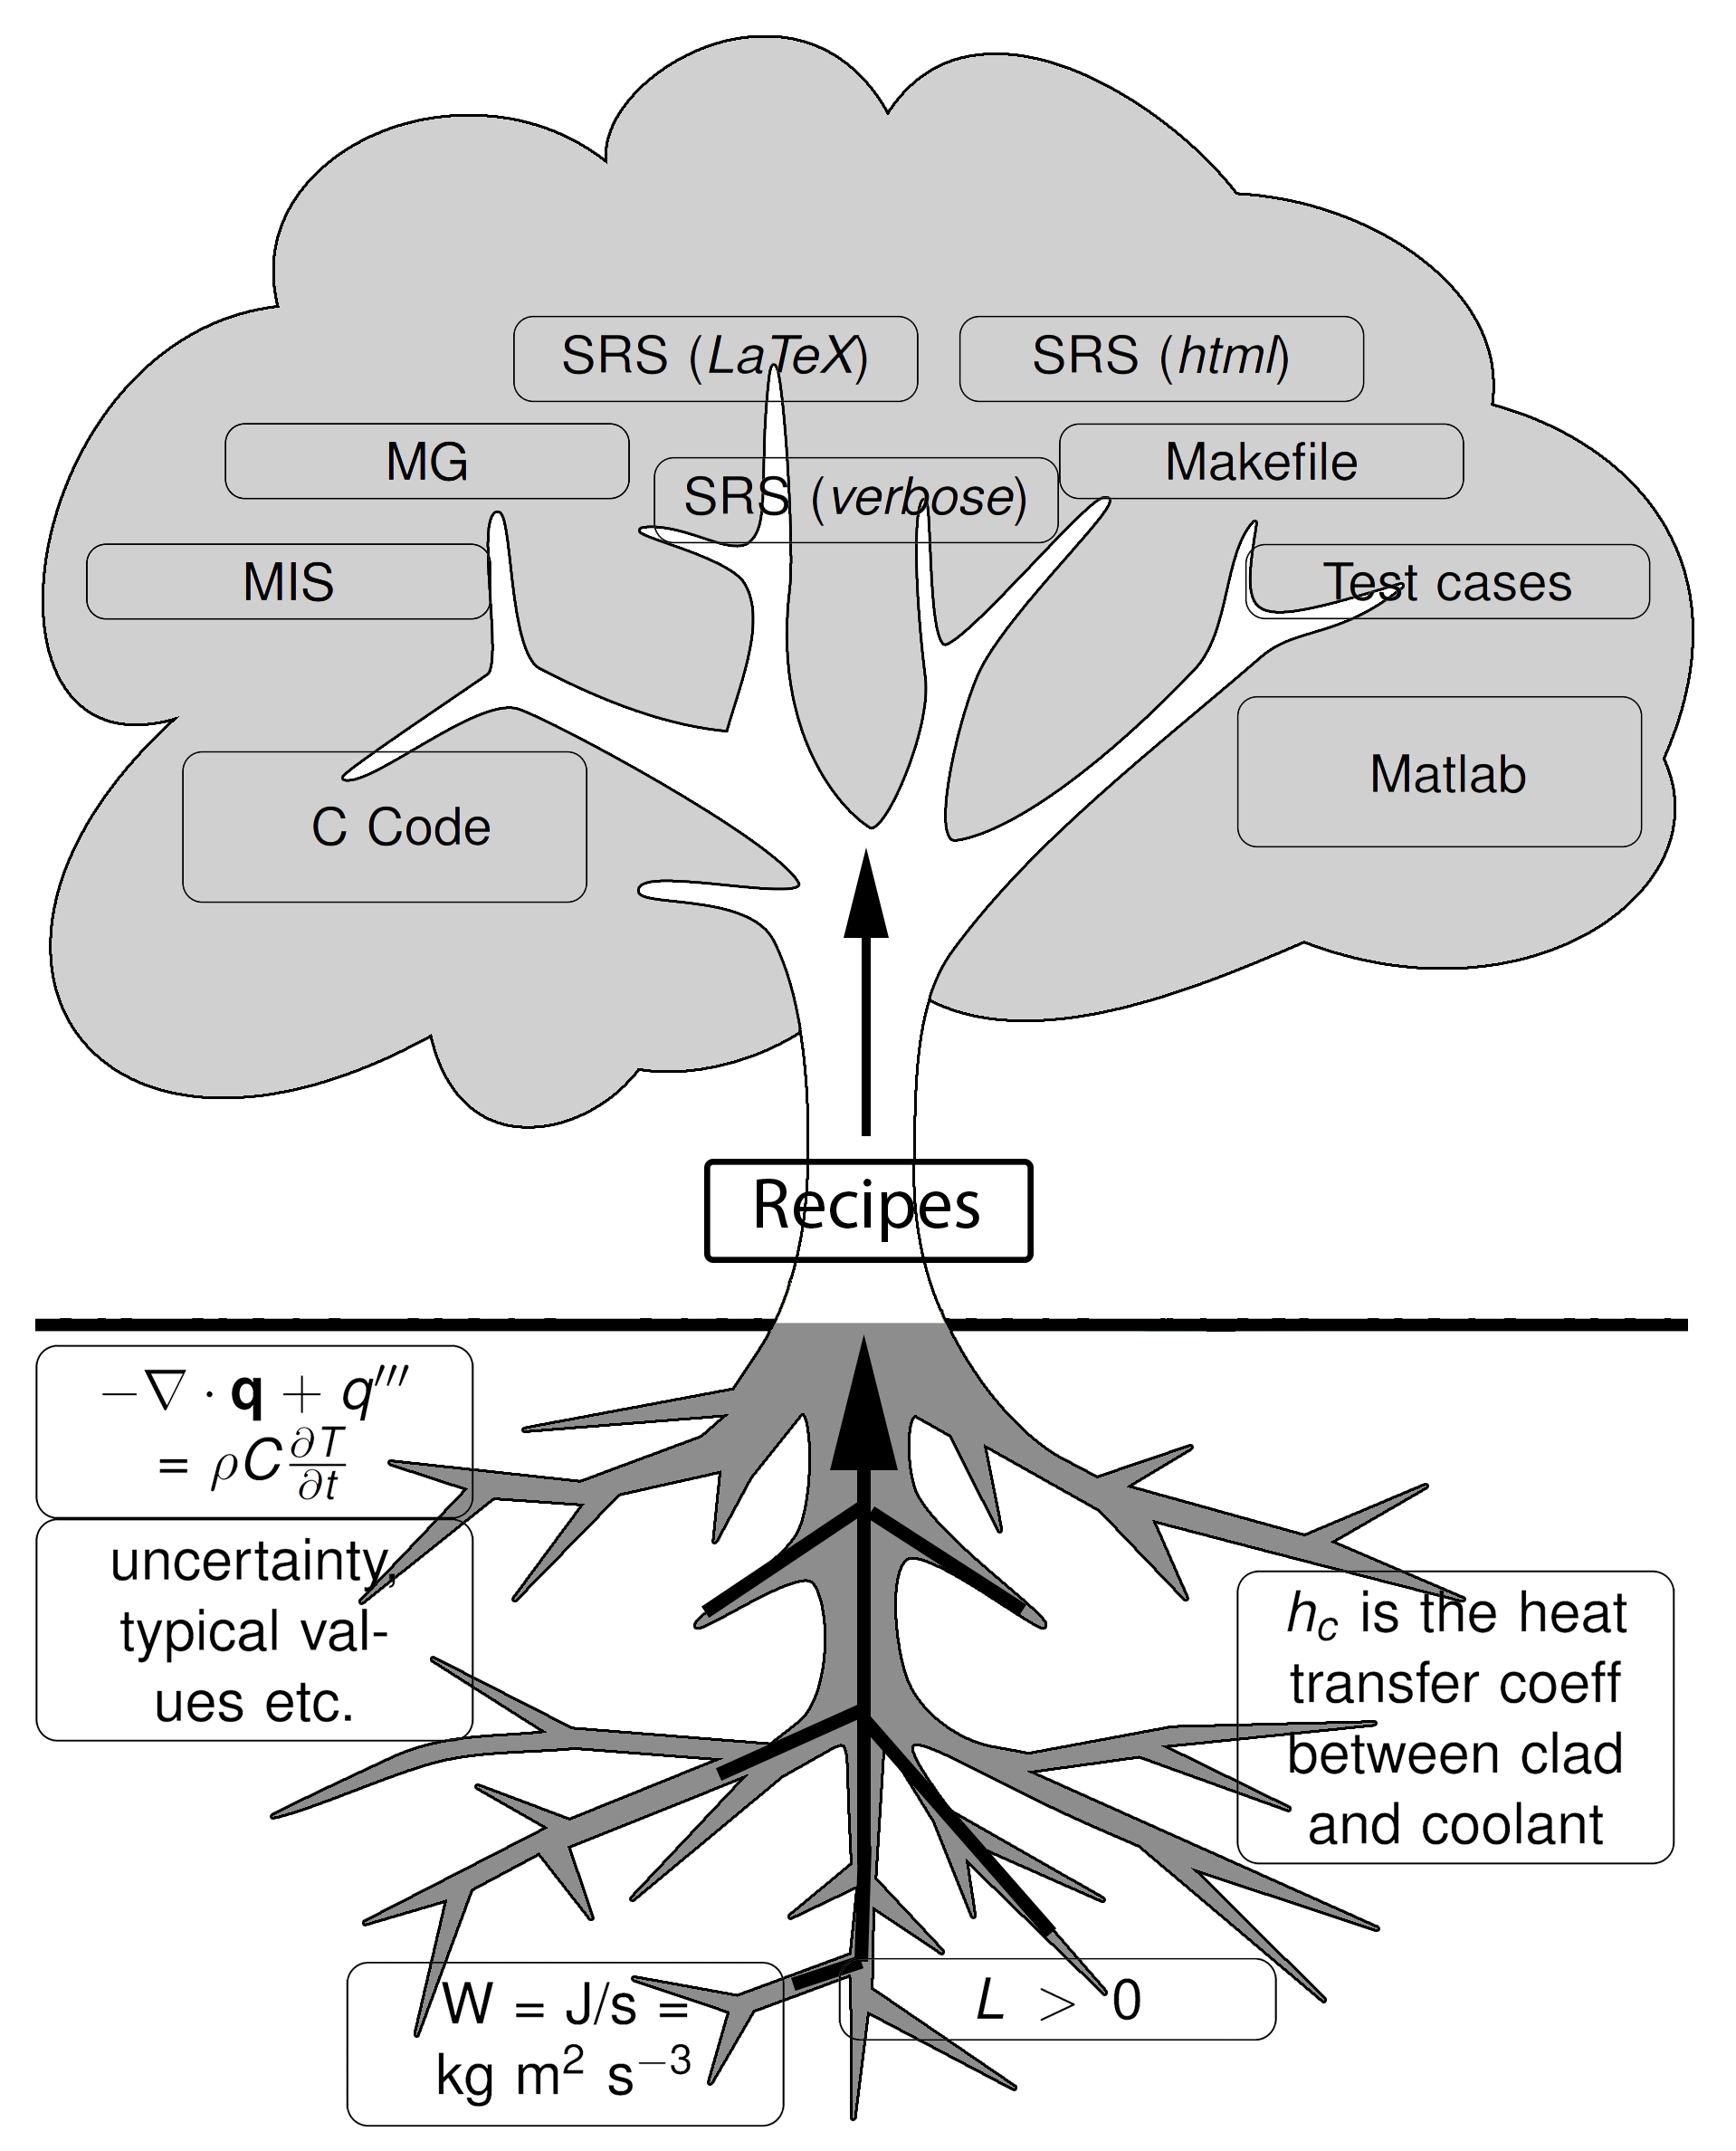
\includegraphics[height=10em]{tree.png}
};
\end{tikzpicture}

\end{frame}

%%%%%%%%%%%%%%%%%%%%%%%%%%%%%%%%%%%%%%

\begin{frame}[allowframebreaks]
\frametitle{References}
\bibliography{CAIMS}
\bibliographystyle{plainnat}
\end{frame}

%%%%%%%%%%%%%%%%%%%%%%%%%%%%%%%%%%%%%%

\end{document}